\chapter{An Overview of Authentication for Computer Communications}

\begin{center}
\uppercase{Dr. H. S. Madhusudhana}

\vskip -6pt

Oracle India Pvt. Ltd.
\end{center}


%~ \bigskip
%~ \noindent\makebox[\textwidth]{
\includegraphics[width=\paperwidth]{src/Figures/bannercoverstoryleft.jpg}}

\newpage

\begin{multicols}{2}

\section*{Abstract}

\noindent
Authentication is the first and foremost security principle that involves validation of identity of an user or a machine. The successful authentication is required for authorization and secure data exchanges. A common classification of authentication system based on factors -- something you know, something you own, something you did and something you are - is explained. Well-known and used password schemes employed in practice is described along with standards. A description Kerberos of authentication system based on symmetric key encryption and SSL based authentication which is based on public key encryption is given. Related Single-Sign-On technologies are explained. A brief overview of authentication for cloud computing, IoT and UIDAI is presented.\\[-22pt]

\section{Introduction}

\vskip -3pt

It is important to know the basic principles of information security as applicable to computer science. This knowledge helps one to develop products with required security and to analyze competing security claims. The first and foremost security principle is ``Authentication", which is the process of verifying the identity of a machine or person. One has to provide valid credentials for successful authentication to get access to computer system resources. The second basic security principle is ``authorization", which controls the access to resources after successful authentication. A common tendency is to combine authentication and authorization, but it is important to understand that they are distinct. The next principles are ``confidentiality'' to provide data protection and ``data integrity'' to assure data is not modified in transit/storage. The related concept of key management is tied with these principles. The final principle is ``availability'' which is to make systems available despite threats and attacks.

The identity of a security principal, either you or a computer, is a declaration of who you are. This is the answer to the question ``Who are you?'' Some common examples of identity are user IDs, digital certificates and ATM cards. The system wants to be certain that it is indeed you and not someone else. The system will challenge the principal and expects correct responses in some way. Common examples of authenticators are passwords, private keys and PINs. Whereas identity is generally public, authentication is private: it's a secret known only by the Principal. A typical scenario is where the client authenticates to the server to get access to service or resource. The case where both parties want to authenticate to each other is called mutual authentication. 

Further, authentication is also applicable to message sent to each other. The receiver wants to be confident that the authentic message is indeed sent by the intended sender and not by someone masquerading as the sender. He also wants to be sure that the message has not been modified in transit. These authentic messages exchanged between the server and the client is the basis for arriving at the common shared key for protected data transfers.

This paper is organized as follows. A common classification of authentication into password, biometric and tokens/certificates is explained. The well-known standards for authentication is highlighted. A different way of classification based on security level is described next. This is followed by a survey of various password based authentication schemes. A description of Kerberos standards follows. The popular SSL based authentication is explained next. Related authentication technologies OpenID and OAuth are explained. A brief survey of authentication for cloud computing IoT and UIDAI is given.

The most common attacks against authentication include impersonation and message tampering. The impersonation attack means the attacker pretending to be a bonafide sender and tricking the receiver to think it has come from the sender. The second attack is to modify the sender's message undetected by the receiver. As and when an authentication method is explained, a description of various attacks/threats handled by the scheme will be given.\\[-22pt]

\section{Common Authentication Methods}

\vskip -3pt

A traditional way to classify is based on the following factors \cite{chap2-key2}:
\begin{quote}
Something you know - Password\\
Something you are - Biometric\\
Something you have - \hbox{Access tokens, Certificates}\\
Something you do - make a gesture, read a text, match a CAPTCHA
\end{quote}

The password is simple to use and remember. It has been used in military since ancient times. A person wishing to enter protected area is to supply a password and he is allowed entry only if the password is correct. Even in modern times, its use is widespread to gain entry into computers, mobile phones, ATM, etc. If the password is formed from multiple words it is called passphrase and if it is formed from numbers, it is called passcode or passkey. A good practice is to choose password which is easy to remember and type but hard to guess \cite{chap2-key2}.

Biometric authentication makes use of many physiological and behavioral characteristics that are believed to be unique to individuals. The identification characteristics is something you are and uniqueness ensures difficulty of forging. A survey of physiological and behavioral characteristics useful for biometric identification are fingerprints, voice, iris, retina, hand geometry, face recognition, signature, key stroke, bio-electric signals, gait, ear shape, head resonance, odor and finger shape is given in \cite{chap2-key3}. A comparative study of these characteristics for biometric authentication system is presented. 

Another type of authentication based on tokens is modeled on a physical key which is restricted to open a room, a building, etc. This type has to do with the ownership. Corporate badges, possession of king's seal, passport and smart cards are other examples. Token verifiers may or may not have readers. In the latter case, the user has a token and can compute the reply to challenge posed by the remote host for authentication. Alternatively, a time-based token calculator, where passwords change regularly and in sync with that on the host. Yet another way is to use One-time passwords. The user has a list of passwords and uses each of them only once \cite{chap2-key2}. The certificate based authentication will be described later.

When only a single method among the preceding options is used, it is called single-factor authentication. Multi-factor authentication uses more than one of the options simultaneously during the authentication process (two-factor uses two, three-factor uses three, and so on) \cite{chap2-key2}. A familiar example of two-factor authentication is the ``sign-on'' process at a banking machine where the user presents a credit or debit card (``something you have'') and enters a PIN (``something you know'') to gain access to his/her bank account. Clearly, multi-factor systems are more burdensome for the user as more tasks are to be completed before the authentication process is finished. However, the security benefit is that impersonation attacks become much more difficult. Another example is online mobile banking transactions where the user is required to provide a password and One-time pseudorandom number received over the mobile (ownership factor).

A biometric system should take into account day-to-day variations in individuals bio-metric and be reliable. Though biometrics characteristics are hard to forge, it is easy to forge after a measurement is taken. An important criterion during biometric authentication is to check for liveliness of the input data. To make biometrics more effective, it is combined with a secret of some kind --- a PIN, a private key on a smart card, or, yes, even a password. In other words biometric characteristic should be treated as pure identity and use other forms for authentication verification.

\section{Standards for Authentication}

If the security technology has not kept pace with rapid development of Information Technology (IT), IT systems, users and data, both organization and private, will be vulnerable to attacks. The attackers could be criminals or politically motivated or financially motivated. Information security standards help to prevent most of the threats, to manage security risks by making it harder for attacks to succeed and by reducing the effects of attacks.

The goal of information security standards is to improve the security of the information systems, to define functional and assurance requirements, to promote vendors to build standard-compliant product, to enable consistency among product developers and to serve as a reliable metric for purchasing products.

Request for Comments (RFC) is a collaborative publication from engineers and computer scientists in the form of a memorandum describing methods, behaviors, research, or innovations applicable to the working of the Internet and Internet-connected systems. The Internet Engineering Task Force (IETF) adopts some of the proposals published as Request for Comments (RFC) as Internet Standards. For authentication methods described here RFC's will be mentioned where applicable.

The US National Institute of Standards and Technology (NIST) publishes white papers and other resources in its Security Management \& Assurance working group. These standards are followed by mainly, US federal agencies. The recommendations are applicable to other organizations as well and referred to as NIST standards.

\section{Password based Authentication\hfill\break Schemes}

The users connect to the network via a remote connection over VPN or dial up network. In this case Password Authentication Protocol (PAP) is used \cite{chap2-key4}. After the user establishes a link, it repeatedly sends his id/password to authenticator. If he receives ACK, the connection is established. If the user receives NAK instead, the connection is terminated. The protocol is simple and the drawback is that the password is sent in the clear text.

Challenge Handshake Authentication Protocol (CHAP) is more secure than the PAP and makes use of a cryptographic hash function such as MD5 or SHA \cite{chap2-key1}. A cryptographic hash is a one-way function takes arbitrary size input and after computations it outputs 128-bit output. The security of the cryptographic hash comes from the fact that given a message ``m'' which hashes to digest ``d'', it is computationally hard to find another message ``m$'$'' that hashes to the same digest ``d''.

RFC 1994 is the standard for CHAP for authentication used by the servers to validate the identity of remote clients \cite{chap2-key5}. Both the server and the client perform a hash operation on the password and transmits the hash result rather than sending the password itself as shown in Figure \ref{chap2-fig1}. After the link is established the server sends a random challenge to the authenticating client entity. The entity responds with hash value calculated using the password and the challenge. The server checks the client response against its own computation and if the values match authentication is successful, else the connection is terminated.
\end{multicols}

\begin{figure}[!ht]
\centering
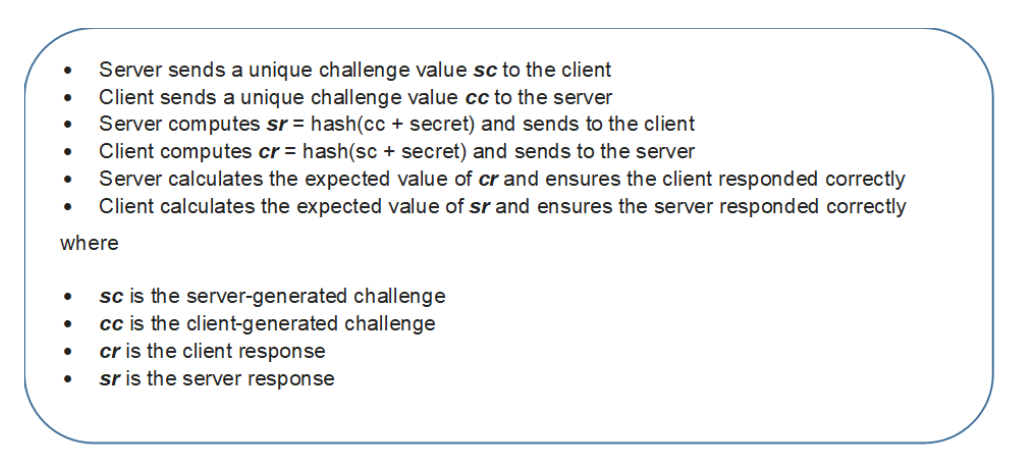
\includegraphics[scale=.85]{src/Figures/chap2/1.eps}
\caption{Challenge Handshake Protocol}\label{chap2-fig1}
\end{figure}

\begin{multicols}{2}
CHAP provides protection against replay attacks through the use of random challenge value. Further the challenge can be used repeatedly to limit the time of exposure for any single attack. If the CHAP negotiations can be carried out in both directions, this results in mutual authentication.

The Microsoft Windows 2000 default authentication is based on the standard CHAP and the latest version is called MS-CHAP v2 \cite{chap2-key4}. It uses two-way authentication so that both the server and the client identities are verified. Like CHAP, MS-CHAP uses challenge-response mechanism to authenticate connection without sending any passwords. The MD4-hashed version of the user password, the peer-challenge string, the session identifier are combined to form SHA hash based response. Other authentication methods related to CHAP is EAP (Extensible Authentication Protocol), and PAP (Password Authentication Protocol) \cite{chap2-key4}.

CRAM-MD5 defined in IETF RFC 2195 \cite{chap2-key6} is a challenge-response authentication mechanism (CRAM) based on the HMAC-MD5 algorithm. HMAC-MD5 is keyed MD5 hash where the key is shared secret. CRAM provides protection against replay attacks. However, it can't prevent cracking the password through a brute-force attack, so it is less effective than alternative mechanisms that avoid passwords or that use connections encrypted with SSL/TLS. 

A more secure Salted Challenge Response Authentication Mechanism (SCRAM) defined in RFC 5802 \cite{chap2-key7} is a family of modern, password-based challenge--response authentication mechanisms providing authentication of a user to a server. In this protocol, both the client and the server exchange their respective nonce and prove to each other the knowledge of the shared secret leading to mutual authentication as shown in Figure \ref{chap2-fig2}. This is an assurance against man-in-the-middle attack. Although all clients and servers have to support the SHA-1, all hashing algorithm and functions defined by the IANA are supported. The main advantage of SCRAM is in storing passwords in data servers in a secure manner to avoid data breaches. The password along with the salt and iteration count are used in Password Based Key Derivation 2 (PBKDF2) algorithm to compute the hashed password. PBKDF2 applies a pseudorandom function to the input password along with a salt value and repeats the process many times to produce a derived key, which can then be used as a cryptographic key in subsequent operations. This makes the computational work for password cracking much more difficult, and is known as key stretching.

Remote Authentication Dial-In User Service (RADIUS) is a networking protocol that provides centralized Authentication, Authorization, and Accounting management for users who connect and use a network service. RADIUS uses two packet types to manage the full AAA process; Access-Request, which manages authentication and authorization defined in RFC 2865 \cite{chap2-key8}; and Accounting-Request accounting, which is described by RFC 2866. RADIUS is often used by Internet Service Providers (ISPs) and enterprises to manage access to the Internet or internal networks, wireless networks, and integrated e-mail services. These networks may incorporate modems, digital subscriber line (DSL), access points, virtual private networks (VPNs), network ports, web servers, etc.

The user or machine sends a request to a Network Access Server (NAS) to gain access to a particular network resource using access credentials. In turn, the NAS sends a RADIUS Access Request message to the RADIUS server, requesting authorization to grant access via the RADIUS protocol. This request includes access credentials, typically in the form of username and password or security certificate provided by the user. Additionally, the request may contain other information which the NAS knows about the user, such as its network address or phone number, and information regarding the user's physical point of attachment to the NAS. 
\end{multicols}

\begin{figure}[!ht]
\centering

\includegraphics[scale=.74]{src/Figures/chap2/2.eps}
\caption{SCRAM Authentication Protocol}\label{chap2-fig2}
\end{figure}

\begin{multicols}{2}
\noindent
The RADIUS server issues ``Access Challenge'' requesting additional information from the user such as a secondary password, PIN, token, or card following PAP, CHAP or EAP \cite{chap2-key9} authentication schemes. Once the user's proof of identification is verified, along with, optionally, other information related to the request, RADIUS send ``Access Accept'' granting access to the user. In case of failure RADIUS returns ``Access Reject'' and the user is unconditionally denied access to all requested network resources.

DIAMETER, developed to provide a framework for AAA to overcome the limitations of RADIUS, is described in RFC 7075 \cite{chap2-key24}. The latter had issues with reliability, scalability, security and flexibility. RADIUS cannot deal effectively with remote access, IP mobility and policy control. The Diameter protocol defines a policy protocol used by clients to perform policy, AAA, and resource control. This allows a single server to handle policies for many services.

DIAMETER provides an upgrade path for RADIUS and provides extra features lacking in RADIUS. It has similar features as RADIUS: it can work in both local and roaming AAA situations; it supports stateful and stateless modes; and it supports application layer acknowledgement and defines failover.

DIAMETER uses TCP or SCTP unlike RADIUS which uses UDP, therefore delegating detection and handling of communication problems to those protocols. DIAMETER does not include encryption, but can be protected by transport level security IPSEC or TLS. Diameter has enhanced features to support many different interfaces defined by 3rd Generation Partnership Project (3GPP) IP Multimedia Subsystem (IMS).

Both RADIUS and Diameter support authentication CHAP and EAP (Extensible Authentication Protocol), and PAP (Password Authentication Protocol). However, RADIUS has some limitations: Its CHAP authentication is subject to dictionary attacks, and it protects clear-text passwords (PAP) only on a hop-by-hop basis. 

\section{Kerberos Authentication Protocol}

Kerberos is an authentication server developed as a part of Project Athena, MIT. According to Greek mythology, Kerberos is a ferocious 3-headed dog guarding the Gates to the Underworld. Since Kerberos authentication requires 3 entities to authenticate and has an excellent track record of making computing safer, the naming is appropriate. 

Kerberos model is based on Needham-Schroeder trusted third party protocol \cite{chap2-key1}. It uses symmetric key cryptography and requires trusted third-party authorization to verify user identities. It provides centralized private-key third-party authentication in a distributed network. The latest Kerberos Version 5 is specified in RFC 4120 \cite{chap2-key12}.

It is highly reliable and employs a distributed server architecture. As it is scalable, the system should support large number of clients and servers. This technology is used by Microsoft Windows, Apple OS, FreeBSD, UNIX and Linux. Kerberos protocol messages are protected against eavesdropping and replay attacks. The strong cryptography and third-party ticket authorization make it much more difficult for attackers to infiltrate the network.

Kerberos system has two main parts Authentication Server (AS) and Ticket Granting Server (TGS) as shown in Figure \ref{chap2-fig3}. Users interact with AS to identify self and negotiate a ticket granting ticket (TGT) which is a non-corruptible authentication credential. Users can subsequently request access to other services from TGS based on the TGT.
\end{multicols}

\begin{figure}[!ht]
\centering
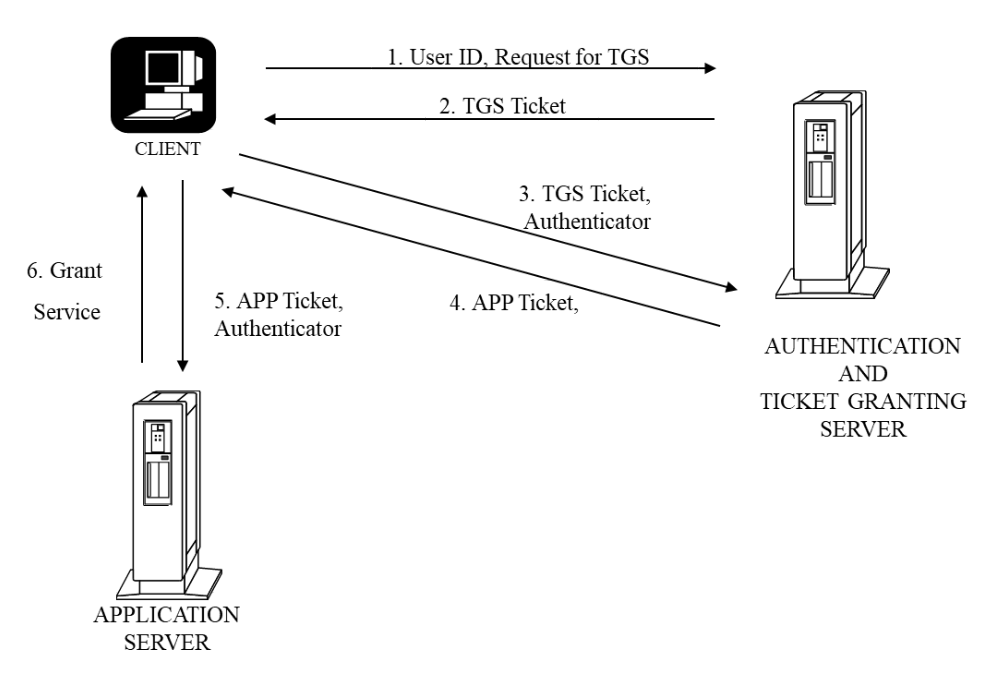
\includegraphics[scale=.82]{src/Figures/chap2/3.eps}
\caption{Kerberos Authentication Mechanism}\label{chap2-fig3}
\end{figure}

\begin{multicols}{2}
Kerberos V5 Messages:
\begin{enumerate}
\item The client sends a clear text message consisting of the user ID and the TGS server name to the AS.
\item The AS checks to see if the client is in its database. If it is, the AS generates and sends back the following two messages to the client:

Message A: Client/TGS Session Key encrypted using the secret key of the client

Message B: Ticket-Granting-Ticket (TGT), which includes the client ID, network address, the server name, a time-stamp and the client/TGS session key encrypted using the secret key of the TGS.

The client decrypts the first message and retrieves the session key. Only the legitimate client with the correct knowledge of the password is able to decrypt the message.

The client saves the session key and TGT for the future use. It erases the password and its one way hash to reduce the chance of compromise.

\item A client sends a request to the TGS to obtain separate tickets for each of the services she wants to use from TGT. The request consists of an authenticator encrypted with the shared session key between the client and the server and TGT. The authenticator consists of the client name, time stamp and optional key. The TGS, upon receiving the request, decrypts the TGT and retrieves the shared session key. Then the shared key is used to decrypt the authenticator. After due validations of the client information from the ticket and the authenticator, the request is allowed to proceed.

Checking timestamps assumes all machines in Kerberos authentication network have synchronized clocks, at least to within several minutes. If the timestamp in the request is too far from the current time, TGS treats the request as an attempt to replay.

\item TGS responds to the valid request by returning a valid ticket for the client to present to the app server along with the new session key for the client and the app server.

\item The client similar to step 3 creates an authenticator for the app server and sends authenticator encrypted with the shared key and the app server ticket.

\item The server decrypts the ticket to retrieve the shared session key and then uses it to decrypt the authenticator. It compares client credentials and timestamp in the ticket as well as authenticator. If everything checks out, the app server grants service access to the client.
\end{enumerate}

Kerberos may be susceptible to replay attacks from old and cached authenticators. Although, the timestamps are used to prevent this, replays are possible during ticket's lifetime. The servers are supposed to store all live tickets to stop this but this is not always practicable. Another requirement is that all the clocks in the network are time synchronized. If a host is fooled about the correct time, old authenticator replay is possible. Yet another vulnerability is password cracking attacks. If the intruder collects enough tickets his chances of success are good.

\section{Public Key Cryptography based\hfil\break Authentication}

Though the use of shared key or symmetric key encryptions is widespread because of its moderate computations, the key distribution and management becomes more unwieldy and complex. If ``n'' users want to securely communicate with each other, this would require ``$(\text{n}^{2}-\text{n})/2$'' secret keys. It is difficult to arrange in advance secure physical means of sharing secret keys for large ``n''. Public key cryptography (PKC) is invented as a solution by Whitefield Diffie and Martin Hellman and independently by Merkle \cite{chap2-key1}, \cite{chap2-key13}. In a PKC system, each user will have only one private key, which should be kept secret and the related public key which can be shared with others.

The generation of private and public keys depends on cryptographic algorithms based on mathematical problems to produce one-way functions. A typical invertible one-way function ``f'' be a function defined over integers modulo a large number N (which can be a prime or product of two large primes) such that computing f(x)=y, given `x' is easy; however, given y=f(x), computing `x' from `y' is difficult or hard. If ``N'' is a single prime, the computation of x given y is termed the discrete logarithm problem \cite{chap2-key1}. If ``N'' is the product of 2 prime numbers, the computation of x given y is equivalent to finding the factors of N, termed the factorization problem \cite{chap2-key1}. The well-known Rivest-Shamir-Adelman (RSA) PKC system, named after its inventors, is based on a number which is product of two large primes \cite{chap2-key14}. Typical operations of encryption and decryption are shown in Figure \ref{chap2-fig4}. 

Two of the best-known uses of public key cryptography are to ensure confidentiality and signature. In the first case, if any one wants to send a message to user A, the message has to be encrypted with the user-A's public key. This encrypted message cannot be decrypted by anyone other than user-A, who does not possess the matching private key. Only the user-A can decrypt the message who is the owner of that key and the person associated with the public key. This is used in an attempt to ensure confidentiality.

Digital signatures, in which a message is signed with the sender's private key and can be verified by anyone who has access to the sender's public key. This verification proves that the sender had access to the private key, and therefore is likely to be the person associated with the public key. This also ensures that the message has not been tampered with, as a signature is mathematically bound to the message it originally was made with, and verification will fail for practically any other message, no matter how similar to the original message.

The security of RSA PKC system is broken if we are able to factorize a large composite integer N. Even though other easier approaches to break RSA are proposed, none of them has held up. Different algorithms for factorization are described in \cite{chap2-key1}. Number Field Sieve (NFS) is the fastest known among these algorithms. Based on these results computational complexity needed to break can be estimated. The NIST recommends 2048-bit keys for RSA to be secure until 2030. An RSA key length of 3072 bits should be used if security is required beyond 2030. 

How a user can authenticate using PKC system? A server can send server-random to the client and the client sends encrypted server-random using its private key. Then the server decrypts the message using the client's public key and allows access if the decrypted message matches the server-random. However, it is not advisable to encrypt arbitrary strings by untrusted parties as an attacker can collect such messages to mount a cipher text attack. Another vulnerability is man-in-the-middle attack, where the attacker can successfully intercept messages and participate in the authentication as a server to the client and as a client to the server.

As we shall see later, Security Socket Layer (SSL) based authentication provides protection against both vulnerabilities. An alternative PKC authentication method requires the client to perform some computation based on random numbers exchanged between the server and the client and the client's private key. To support such authentication protocols, a variant RSA system based on quadratic residue is needed and described in \cite{chap2-key1}. However, such systems are not in wide use. 

The main problem in PKC is how to get some one's public key in a secure way to avoid substitution by attackers. A solution is possible if the user's public key along with their name, address and so on is signed by a trustworthy person. This credential binding between a public key and subject's identity is called a digital identity or public key certificate. It is signed by Certification Authorities (CA). A public key infrastructure (PKI) is a system for the creation, storage, distribution and revocation of digital certificates which are used to verify that a particular public key belongs to a certain entity. 

There are various roles within PKI. It consists of a certificate authority (CA) that stores, issues and signs the digital certificates, a registration authority (RA) which verifies the identity of entities requesting their digital certificates to be stored at the CA, a central directory to store and index keys, a certificate management system for managing certificates and a certificate policy stating the PKI's requirements concerning its procedures. The most common format for public key certificates is X.509 as defined in RFC 5280 \cite{chap2-key15}.

{\parfillskip=0pt
There is a certificate chain of trust in validating a digital certificates. Three CA's Symantec, Comodo, GoDaddy dominate the CA market issuing certificates to nearly 75\% of web servers. These CA's or their trusted agents certify organization CA which in turn certify their employees. SSL/TLS operation use certificates signed by issuer CA, which is the basis for centralized key management. Alternatively, Pretty Good Privacy (PGP) uses distributed key management to solve the trust problem with the concept\par}
\end{multicols}

\begin{figure}[!ht]
\centering
\includegraphics[scale=.9]{src/Figures/chap2/4.eps}
\caption{Typical RSA Encryption and Decryption}\label{chap2-fig4}
\end{figure}

\begin{multicols}{2}
\noindent
of introducers \cite{chap2-key1}. A user-A can get his certificate signed by his friends, say user-B and user-C, also called introducers. Suppose the user-A wants to connect with the user-D, with whom he does not have any acquaintance; so the user-A presents his introducer certificates to the user-D. If the user-D either trusts user-B and/or user-C, then the user-A certificate is acceptable to him.

The certificate has an indication of validity period for its use. However, a certificate may be invalidated before expiry date either due to compromise or due to administrative reasons. So CA should keep a list of revoked certificates and the users to regularly check that list.

\section{SSL/TLS Authentication Protocol}

Transport Layer Security (TLS), and its now-deprecated predecessor, Secure Sockets Layer (SSL) are cryptographic protocols designed to provide confidentiality and data integrity between a client (e.g., a web browser) and a server (e.g., amazon.com). Websites can use TLS to secure all communications between their servers and web browsers. The connection established by TLS/SSL protocol is secure because symmetric key is used for data encryption. The keys are uniquely generated for each connection based on shared secret negotiated during the handshake. The protocol ensures that the shared secret is protected against eavesdrop and man-in-the-middle attack. The authentication is provided by PKC and server's trusted certificates. The connection is reliable as the message integrity is provided using cryptographic hash.

TLS involves many configurable parameters and supports many different methods for exchanging keys, encrypting data, and authenticating message integrity. TLS is a proposed Internet Engineering Task Force (IETF) standard, first defined in 1999 and updated in RFC 5246 \cite{chap2-key16}.

Figure \ref{chap2-fig5} shows the messages in a typical TLS protocol. A client connects to a TLS-enabled server requesting a secure connection by sending the ClientHello message which includes ClientRandom and a list of supported cipher suites and hash functions. The server sends ServerRandom in the ServerHello message. Then the server picks a cipher and hash function that it also supports and notifies the client of the decision. The server usually then provides identification in the form of a digital certificate, which contains the server name, and trusted certificate authority (CA) that vouches for the authenticity of the certificate, and the server's public encryption key. The client confirms the validity of the certificate before proceeding. The generation of the shared session key is done as follows. The client encrypts a premaster secret with the server's public key and sends the result to the server; both parties then use the ServerRandom, ClientRandom and the premaster secret to generate unique session keys for subsequent encryption and decryption of data during the session.

The most common use of certificates is for HTTPS-based web sites. A web browser validates that an HTTPS web server is authentic, so that the user can feel secure that his/her interaction with the web site has no eavesdroppers and that the web site is who it claims to be. This security is important for finance and business applications. A web site operator obtains a certificate by applying to a certificate authority with a certificate signing request. The certificate request is an electronic document that contains the web site name, company information and the public key. The certificate provider signs the request, thus producing a public certificate. During web browsing, this public certificate is served to any web browser that connects to the web site and proves to the web browser that the provider believes it has issued a certificate to the owner of the web site.

A certificate provider has options to issue three types of certificates, each requiring its own degree of rigor, namely, Domain Validation, Organization Validation and Extended Validation. A certificate provider will issue a Domain Validation (DV) class certificate to a purchaser if the purchaser can demonstrate the right to administratively manage a domain name. An Organization Validation (OV) class certificate will be issues to a purchaser if the purchaser has the right to administratively manage the domain name in question, and based on some vetting of organization's actual existence as a legal entity. To acquire an Extended Validation (EV) certificate, the purchaser must persuade the certificate provider of its legal identity, including manual verification checks by a human.
\end{multicols}

\begin{figure}[!ht]
\centering
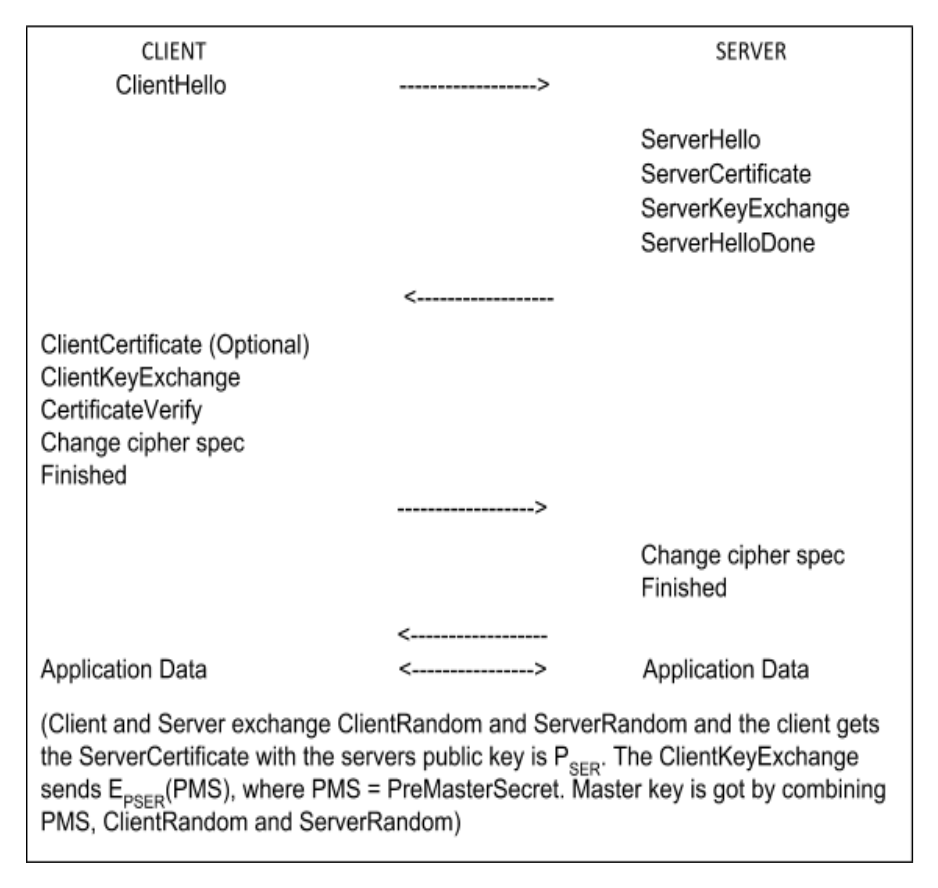
\includegraphics[scale=.75]{src/Figures/chap2/5.eps}
\caption{TLS Protocol Messages}\label{chap2-fig5}
\end{figure}

\begin{multicols}{2}
Browsers will generally offer users a visual indication of the legal identity when a site presents an EV certificate. Most browsers show the legal name before the domain, and use a bright green color to highlight the change. In this way, the user can see the legal identity of the owner has been verified.\\[-22pt]

\section{Related Authentication Technologies}

\vskip -3pt

A typical user in an enterprise can access multiple applications: one, for example, to create expense reports, another to use email, and so on. Each application requires the user to enter a valid user name and password to access the services. One of the problems is that it is inconvenient for the user to remember password for multiple applications. This makes user to use the same password or writing it on a piece of paper. In both cases the chances of password being compromised is high. Also, it can be costly and difficult to administer password stores for multiple applications. To help alleviate these problems, enterprises provide Single-Sign-On (SSO) capability for a user to log in with a single ID and password to gain access to multiple related, yet independent systems. From user's perspective, the user needs to enter his credentials only once at a central corporate web portal and authentication to all the needed applications happen transparently \cite{chap2-key19}.

As different applications support different authentication mechanisms, SSO must internally store the credentials used for the initial authentication and translate them to the credentials required for the different applications. As SSO requires an increased focus on the protection of the user credentials, it should ideally be combined with strong authentication methods like smart cards, certificates and one-time password tokens. If the initial sign-on prompts the user for the smart card, additional software applications can also use the smart card, without prompting the user to re-enter credentials. Smart-card-based single sign-on can either use certificates or passwords stored on the smart card. Enterprise security features being offered by the SSO system critically depends on good governance of the underlying identity data. Therefore, most modern single sign on systems use LDAP (Lightweight Directory Access Protocol) directories to store the authentication and authorization policies. The LDAP directories provide for new identity creation, identity termination or role changes. Further, doing single authentication to LDAP server helps to gain access to multiple applications by passing the authentication token seamlessly to configured applications \cite{chap2-key20}.

SSO can facilitate cross enterprise authentication using federated login between enterprise-A and enterprise-B using Security Assertion Markup Language (SAML). SAML is an XML-based solution for exchanging user security information between an SAML identity provider and a SAML service provider. SAML 2.0 supports W3C XML encryption and service provider initiated web browser SSO exchanges. An employee from enterprise-B can log on to their SSO and then click on a link to connect to enterprise-A's application. Enterprise-B SSO system will provide a security assertion token to your enterprise using SAML token. Enterprise-A SSO system receives the token, checks it, and then allows access to enterprise-B employee without having to sign on. Similarly, SSO federated authentication also works with enterprise-A employee, who is trying to access outsourced benefits supplier system by clicking on the benefits link. Enterprise-A's SSO system would then send a security assertion token to the benefits supplier. The benefits supplier's SSO system would then take the token, check it and grant access to the employee without making them sign on.

The main benefit from SSO is the ability to enforce uniform enterprise authentication and/or authorization policies across the enterprise and to enable user audit sessions to improve security reporting and auditing. The administrative benefit is to reduce IT costs due to lower number of IT help desk calls about password management. Single Sign-On provides centralized provisioning and administration of user accounts. However, centralized SSO systems, if not available, can become a single point of failure resulting in productivity loss. Therefore, it is essential that your enterprise SSO system have a good and well tested failover and disaster recovery design.

\section{OpenID and OAuth}

OpenID is an open standard and decentralized authentication protocol, works in a way similar to SSO authentication system. It allows users to be authenticated by co-operating sites, known as Relying Parties (RP), using a third-party service, eliminating the need for webmasters to provide their own ad hoc login systems, and allowing users to log into multiple unrelated websites without having to have a separate identity and password for each. Users create accounts by selecting an OpenID identity provider, and then use those accounts to sign onto any website that accepts OpenID authentication. Many websites including Microsoft, Google, AOL, and Amazon have integrated OpenID consumer support.

The OpenID standard provides a framework for the communication that must take place between the identity provider and the RP. An extension to the standard facilitates the transfer of user attributes, such as name and gender, from the OpenID identity provider to the RP. The OpenID protocol does not rely on a central authority to authenticate a user's identity. Moreover, neither services nor the OpenID standard may mandate any specific means by which to authenticate users. It can support commonly used password mechanisms as well as smart cards or biometrics.

An end-user is the entity that wants to assert a particular identity. A RP is a web site or application that wants to verify the end-user's identifier. An OpenID provider (OP) is a service that specializes in registering OpenID URLs or XRIs. OpenID enables an end-user to communicate with a relying party. This communication is done through the exchange of an identifier or OpenID, which is the URL or XRI chosen by the end-user to name the end-user's identity. An identity provider provides the OpenID authentication.

An end-user typically registers with an OpenID provider (e.g. openid.example.org). Then the end-user interacts with a RP that provides an option to specify an OpenID for the purposes of authentication. There are two modes in which the RP may communicate with the OpenID provider. The ``checkid\_immediate'' mode does not require the OpenID provider to interact with the end-user. All communication is relayed through the end-user's user-agent without explicitly notifying the end-user. The second ``checkid\_setup'' mode requires that the end-user authenticate directly with the OpenID provider via the end-user's user-agent used to access the RP. The method of authentication may vary, but typically, an OpenID provider prompts the end-user for a password or some cryptographic token, and then asks whether the end-user trusts the RP to receive the necessary identity details. If the end-user declines the OpenID provider's request to trust the RP, the authentication is rejected. If the end-user accepts the OpenID provider's request to trust the RP, then the user-agent is redirected back to the RP along with the end-user's credentials. If the RP and OpenID provider have established a shared secret, then the RP can validate the identity of the OpenID provider by comparing its copy of the shared secret against the one received along with the end-user's credentials. After the OpenID has been verified, authentication is considered successful and the end-user is considered logged into the RP. The RP typically then stores the end-user's OpenID along with the end-user's other session information.

The OpenID has security weaknesses and may prove vulnerable to phishing attacks. For example, a malicious relying party may forward the end-user to a bogus identity provider authentication page asking that end-user to input their credentials. On completion of this, the malicious party could then have access to the end-user's account with the identity provider, and then use that end-user's OpenID to log into other services. In an attempt to combat possible phishing attacks some OpenID providers mandate that the end-user needs to be authenticated with them prior to an attempt to authenticate with the RP.

OAuth is an open standard for access delegation, commonly used as a way for Internet users to grant websites or applications access to their information on other websites but without giving them the passwords. This mechanism is used by companies such as Amazon, Google, Facebook, Microsoft and Twitter to permit the users to share information about their accounts with third party applications or websites. The standard OAuth 2.0 Authorization Framework is defined in RFC 6749 \cite{chap2-key26}.

The client requests an access to protected resource on the server by using the resource owner's credentials. To facilitate access to restricted resources, the resource owner is required to share its credentials with the third party. This creates several problems and limitations. The credential is a password in clear text needed to be stored in third-party applications and to be supported by the server creating a security vulnerability. Resource owners can neither restrict nor revoke access to third-party. OAuth addresses these issues by introducing an authorization layer and separating the role of the client from that of the resource owner. In OAuth, the client requests access to protected resources is issued a different set of credentials, called access token -- a string denoting a specific scope, lifetime, and other access attributes. Access tokens are issued to third-party clients by an authorization server with the  approval of the resource owner. The client uses the access token to access the protected resources hosted by the resource server. OAuth 2.0 is the industry-standard protocol for authorization described in RFC 6749 \cite{chap2-key21}.

OAuth is an authorization protocol, rather than an authentication protocol. Using OAuth on its own as an authentication method may be referred to as pseudo-authentication. 
\medskip

The communication flow in both processes is similar:
\begin{enumerate}
\item The user requests a website login from the application.
\item The website formulates a request for the identity provider, encodes it, and sends it to the user as part of a redirect URL.
\item The user's browser requests the redirect URL for the identity provider, including the application's request. The identity provider authenticates the user by requesting users' credentials. After successful authentication, it processes the application's request, formulates a response, and sends that back to the user along with a redirect URL back to the application.
\item The user's browser requests the redirect URL that goes back to the application, including the identity provider's response. The application decodes the identity provider's response, and carries on accordingly. 
\end{enumerate}

The crucial difference is that in the OpenID authentication use case, the response from the identity provider is an assertion of identity; while in the OAuth authorization use case, the response from the identity provider is an access token that may grant the application ongoing access to some of the identity provider's APIs, on the user's behalf. The access token acts as a kind of ``valet key'' that the application can include with its requests to the identity provider, which prove that it has permission from the user to access those APIs. Because the identity provider typically, but not always, authenticates the user as part of the process of granting an OAuth access token, it's tempting to view a successful OAuth access token request as an authentication method itself.

However, because OAuth was not designed with this use case in mind, making this assumption can lead to major security flaws.

Similar to OpenID, the most devastating OAuth security failure is phishing vulnerability. An attacker website can visually seem as a genuine website to steal credentials from unsuspecting users.

\section{Authentication for Cloud Computing}

Cloud computing and storage provides users with capabilities to store and process their data in third-party data centers. It provides on-demand availability of services such as software, platform, and infrastructure through Software-as-a-Service (SaaS), Platform-as-a-Service (PaaS) and Infrastructure-as-a-Service (IaaS). This involves using of shared infrastructure and rapid movement of servers and workload within the infrastructure. 

Because of the structure of Cloud computing, both the security issues faced at cloud service provider and security issues faced by cloud customers need to be taken into account.

As cloud service providers often store more than one customer's data on the same server, it is possible that one user's private data can be viewed by other users. The extensive use of virtualization in implementing cloud infrastructure brings unique security concerns for the customers of a public cloud service. The underlying components of cloud infrastructure may not be designed to offer strong isolation properties for a multi-tenant architecture. A virtualization hypervisor mediates access between guest operating systems and the physical compute resources. However, any flaw in hypervisors enable guest operating systems to gain inappropriate levels of control leading to compromise. The cloud service provider should ensure proper data isolation, logical storage segregation and that the virtualization must be properly configured, managed and secured. Strong compartmentalization should be employed to ensure that individual customers do not impact the operations of other tenants running on the same cloud provider.

When an organization opts to use cloud storage, potentially sensitive customer data is at risk from insider attacks. The cloud service provider promotes his service by simplifying registration process and offering free limited trial periods. By abusing the relative anonymity behind these registration and usage models, spammers, malicious code authors, and other criminals have been able to break into PaaS and IaaS services. 

The cloud users must take measures to safeguard their application and use strong passwords and authentication measures. Strong authentication of cloud users makes it less likely that unauthorized users can access cloud systems, and more likely that cloud users are positively identified. Cloud Computing providers expose a set Application Programming Interface (APIs) that the customers can use to provision, manage, orchestrate and interact with cloud services. The security and availability of general cloud services is dependent upon the security of these basic APIs. These interfaces must be designed to protect against both accidental and malicious attempts to circumvent policy.

It is generally recommended that information security controls be selected and implemented according and in proportion to the risks, typically by assessing the threats, vulnerabilities and impacts. Cloud Access Security Broker (CASB) is a software that sits between cloud users and cloud applications to provide visibility into cloud application usage, data protection and governance to monitor all activity and enforce security policies. It is either on-premises or cloud based software that sits between cloud service users and cloud applications, and monitors all activity and enforces security policies. 

A survey of authentication methods used in cloud environment is given in \cite{chap2-key18}. One type of authentication based on cryptographic techniques need a trusted third party using tickets or certificates based on Kerberos or PKI system. The user profile type makes use of either biometrics-based or behavior-based system. Biometrics include finger prints, retinal scan and face recognition methods. Behavioral methods involves handwriting and keystroke based authentication. The biometric data is linked to the confidential information of the users and stored in an encrypted fashion. Making use of a searchable encryption technique, biometric identification is performed in encrypted domain to make sure that the cloud provider or potential attackers do not gain access to any sensitive data or even the contents of the individual queries. Typically, every enterprise will have its own identity management system infrastructure. Cloud providers can integrate the customer's identity management system into their own infrastructure, using federation or SSO technology or a biometric-based identification system.

\section{Authentication for IOT}

Internet of Things (IoT) is a terminology used for a network of low-cost and low-power devices used for sensing and actuating in day to day life. A heterogeneous system combining sensors and actuators with general purpose computing elements consisting of hundreds to thousands of nodes. These devices are deployed globally and can collect various data and actuate or perform specific actions automatically with minimal human interaction.

IoT devices can be deployed to create smart cities, smart grids, smart logistics, etc. IoT devices are also termed as constrained devices because they have limited computational capacity, lifetime, throughput, etc. Sensor nodes form multi-hop wireless network with aggregation capability and sensors communicate with the nearest base station. 

IoT brings with itself unlimited opportunities as well as tremendous challenges. A main challenge is different devices utilize different protocols and standards in their network and these networks need to communicate with each other securely as well as efficiently. From a security point of view, attackers find it convenient to exploit constrained devices and use them to mount DDoS attacks. Standard network security protocols cannot be used for IoT because they need high computational complexity. So, there is a requirement of light weight security protocols for IoT environment.

No standards for IoT authentication schemes have been proposed so far. Various schemes are proposed based on the centralized servers for mutual authentication using different primitives. The authentication scheme proposed by Amin et al. is described in some detail highlighting the kind of cryptographic operations \cite{chap2-key22}.

Amin et al. proposed light weight authentication method in distributed cloud environment \cite{chap2-key19}. Their scheme is based on a central control server for several cloud servers providing control sequence for authentication in a distributed environment as shown in Figure \ref{chap2-fig6}. This scheme makes use of the smart card and based on hash function \cite{chap2-key23}.

Both the cloud server and the client have to perform registration as shown in Figure \ref{chap2-fig7} and Figure \ref{chap2-fig8}. The cloud server sends the server identity, ServID and the random ``d''. The Control Server (CS) uses hash function h() and uses its own secret ``y'' to compute BSm and the cloud server stores BSm and ``d''.

The user registration uses the password Pi, random b1 and b2, computes Ai and PIDi and sends it to the CS. The CS uses its secret x to compute Di and sends $\langle$ci, Di, Ei$\rangle$. The smart card computes DP=h(UIDi||pi) xor b2 saves $\langle$ci, Ei, bb, DP$\rangle$. The user sends IDi and the password Pi the smart card and it computes c'i and if tallies with ci, proceed to choose a random 128-bit ``Ni'' and computes  $\langle$Gi, Fi, Zi, PIDi, TSi$\rangle$ to the server where TSi is the time stamp. The server chooses random Nm and computes Jm=BSm xor Nm and ``km=h(Nm||BSm||Gi||TSm)'' and sends $\langle$Jm, km, PSIDm, Gi, Fi, Zi, PIDi, TSi, TSm$\rangle$ to the central server. The central server computes D'i as it knows its own secret ``x''. Next ``D'i'' is computed and ``N'i'' recovered to find SID'm. The final ``G'i'' is obtained by hashing the concatenated messages. If G'i matches Gi, the central server finds N'm and computes ``k'm''. If ``km'' matches ``k'm'' the authentication is considered successful. It next proceeds to computing session keys to be used for the session.

Amin et al. show that their scheme provides user anonymity, session key agreement, mutual authentication as well as early wrong password detection. They also show that their scheme is secure against off-line password guessing attack, insider attack, user impersonation attack, session key disclosure attack and replay attack. This scheme uses a centralized control server for the flow of authentication data and provides mutual authentication between all the entities. As we can see mutual authentication occurs between the user, the cloud and the control server, it is evident that the chances of a DoS or DDoS attack increases significantly. In Amin et al.'s scheme, if the centralized control server failure is a single point of failure. However, Amin et al. provides no genuine countermeasure for avoiding a DoS attack.

There are other authentication schemes making use of centralized servers for authentication. Huang et al. describe an authentication method using one-way accumulator, which is a one-way hash function that has quasi-communicative property and uses IoT nodes and a proxy server \cite{chap2-key22}. Another authentication using an elegant variation of Lamport's One-Time-Password (OTP) and identity based elliptic curve cryptography is given in \cite{chap2-key22}.
\end{multicols}

\begin{figure}[!ht]
\centering
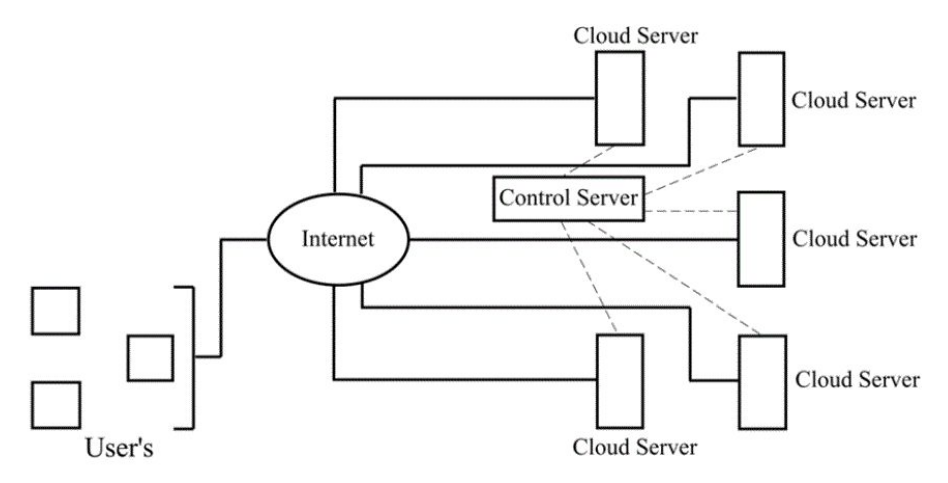
\includegraphics[scale=.77]{src/Figures/chap2/6.eps}
\caption{Cloud Network Architecture for a typical IoT authentication}\label{chap2-fig6}
\end{figure}

\medskip

\begin{figure}[!ht]
\centering
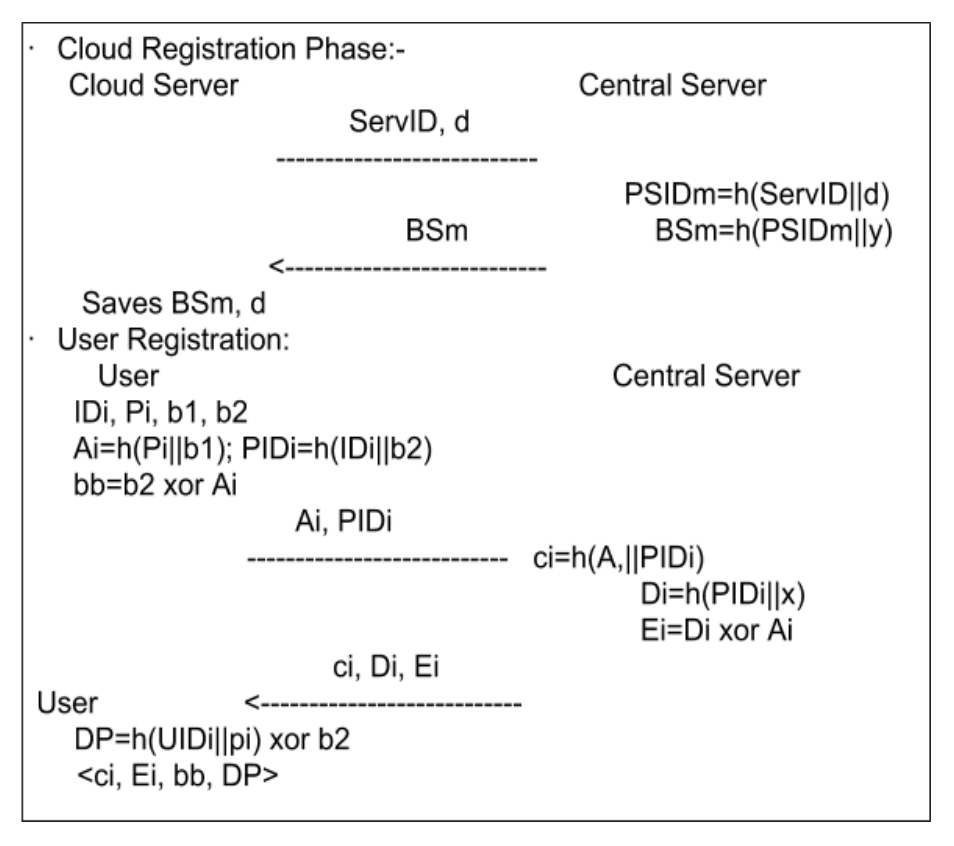
\includegraphics[scale=.7]{src/Figures/chap2/7.eps}
\caption{Server and User Registration in \cite{chap2-key20}}\label{chap2-fig7}
\end{figure}

\newpage

\begin{figure}[!ht]
\centering
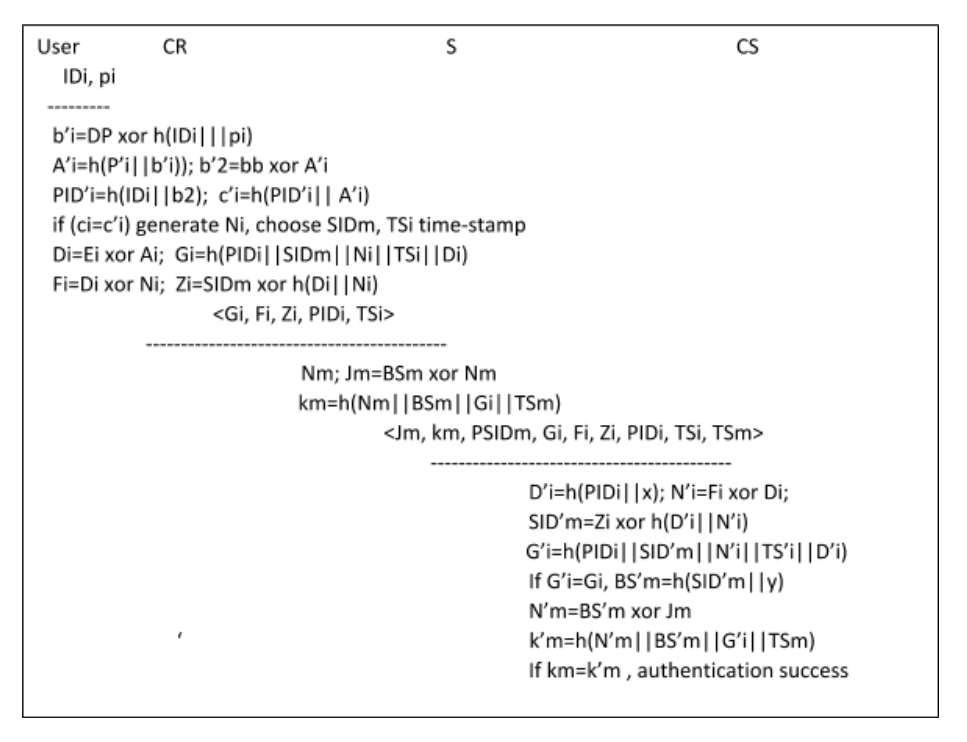
\includegraphics[scale=.85]{src/Figures/chap2/8.eps}
\caption{Cloud authentication by Amin et al. \cite{chap2-key20}}\label{chap2-fig8}
\end{figure}

\begin{multicols}{2}
\section{Authentication in Unique Identification Authority of India (UIDAI)}

UIDAI has been created with the objective to issue Unique Identification numbers (UID), named as ``Aadhaar'', to all residents of India that is (a) robust enough to eliminate duplicate and fake identities, and (b) can be verified and authenticated in an easy, cost-effective way. UIDAI is responsible for Aadhaar enrolment and authentication and also required to ensure the security of identity information and authentication records of individuals. The unique Aadhaar identity enables the Government of India to directly reach residents of the country in delivery of various subsidies, benefits and services by using the resident's Aadhaar number only.
 
The UIDAI has set up a scalable ecosystem for the purpose of instant authentication of residents. The Aadhaar authentication ecosystem is capable of handling tens of millions of authentications on a daily basis, and can be scaled up further as per the demand. The UIDAI has appointed a number of Authentication Service Agencies (ASAs) and Authentication User Agencies (AUAs) from various Government and non-Government organizations. AUA is an organization or an entity using Aadhaar authentication as part of its applications to provide services to Aadhaar holders. All AUAs (Authentication User Agencies) must be registered within Aadhaar authentication server to perform secure authentication.  ASA is an organization or an entity providing connectivity using private secure network to UIDAI's data centers for transmitting authentication requests from various AUAs.
 
UIDAI defines ``Aadhaar Authentication'' as a process by which the Aadhaar number along with demographic information (such as name, date of birth, gender etc.) or biometric information (Fingerprint or Iris) of an individual is submitted to UIDAI's Central Identities Data Repository (CIDR) for its verification and UIDAI verifies the correctness of the details submitted, or the lack thereof, on the basis of information available with it.
 
\vskip -2pt

Aadhaar authentication service is exposed as stateless service over HTTPS. Usage of open data format in XML and widely used protocol such as HTTPS allows easy adoption and deployment of Aadhaar authentication. It is mandated that user's identity data to be encrypted at the time of capture and must not be stored for security reasons. It is essential that ASA and AUA should maintain audit records of authentication transactions and should validate TLS certificates against revocation list online. Aadhaar authentication uses XML as the data format for input and output. UIDAI requires AUA and ASA should digital sign authentication request messages in XML format. This assures message security and integrity. AUA can digitally sign after forming the input XML. ASA can digitally sign the request XML if it is a domain-specific aggregator and forms the request XML on behalf of the AUA.

\vskip -2pt
 
Aadhaar authentication supports authentication using multiple factors. These factors include demographic data, biometric data, PIN, OTP, possession of mobile, or combinations thereof. Adding multiple factors increases the strength of authentication. Applications using Aadhaar authentication need to choose appropriate authentication factors based on risk level of the transaction. AUAs can add their own factors to strengthen authentication.
 
A typical authentication flow and is a case of an operator assisted transaction at a PoS terminal:
\begin{itemize}
\item[a)] Aadhaar holder provides Aadhaar Number, necessary demographic and biometric details to the terminal device belonging to the AUA.
\item[b)] The device packages these input parameters as a Personal Identity Data (PID) block, encrypts it, and sends it to AUA server.	
\item[c)] AUA server, after validation, adds necessary headers such as AUA specific wrapper XML with signature and passes the request through ASA server to UIDAI CIDR.	
\item[d)] Aadhaar authentication server returns a ``yes/no'' based on the match of the input parameters.
\item[e)] Based on the response from the Aadhaar authentication server, AUA conducts the transaction.
\end{itemize}

\section{Conclusion}

A good metaphor for authentication is how we recognize each other. When we meet in person, or talk over the phone or see pictures of each other, how we are able to recognize our close friend. The recognition is so natural and automatic that we don't know what goes on inside the brain. We bring in additional support from our memories and are certain that the person is indeed our closest friend. If someone tries to impersonate as a closest friend, we will be on our guard and watchful that something fishy is going on. Computer machines and systems should emulate ``human authentication'' to the best possible extent.

Traditionally, authentication methods are classified into something you know (password), something you have (tokens), something you did (behavioral) and something you are (biometric). Password is the simplest of these methods and biometric/behavioral are complex to implement. We can combine these methods to obtain multi-factor authentication to get better security. Banking over Internet is a good example that requires both the PIN and the credit card. A brief overview of biometric system is described. It is useful to consider biometrics as an unforgeable identity and use it in combination with encryption to perform a strong authentication. Of late behavioral metrics such as handwriting, keystrokes are receiving more attention to identify unique identity trait. These methods come in handy for systems that need continuous authentication.

Despite security weakness, password methods are popular and widely used. It is mandated that the password must not be transmitted in clear text. CHAP protocol avoids sending the password in clear text and uses challenge-response mechanism to avoid replay attacks as well as to assure mutual authentication. Related PAP, EAP and MSCHAP protocols are mentioned. CRAM-MD5 uses hashed passwords and challenge response mechanisms to prevent replay attacks. However, it is susceptible to offline dictionary attacks. To circumvent this, SCRAM protocol based on salt and iteration is described. A brief account of RADIUS and DIAMETER AAA protocols is presented.

An explanation of Kerberos based on trusted Ticket Granting server is given. Kerberos provides better security but requires time synchronization requirement across the network. PKC based enhancements are being proposed to improve the security.

A brief overview of PKC is given and authentication schemes based on PKC are described. The operations of encryption and decryption in RSA is explained. The user is required to prove his knowledge of private key to the server. To avoid man-in-the-middle attack and to bind the private key to the user's identity, it is required that trusted third party, Certificate Authority, sign the user's certificates. The well-known TLS protocol is explained. Various kinds of SSL certificates and their significance are explained.

To avoid memorizing and entering multiple credentials, SSO authentication is described when logging into an enterprise and accessing many application servers. A secure implementation of SSO requires that enterprise user's identities be strongly protected in a secure directory. Related OpenID and OAuth technologies are described. An overview of cloud architecture is given with security concerns. The role of authentication to mitigate security threats and vulnerabilities is explained and various authentication methods used are given. Finally, a brief overview of authentication in a IoT network of sensors and actuators with limited power and computational capabilities is given. An explanation of authentication method using centralized server is presented. Finally, a brief explanation of UIDAI authentication is given.

While explaining the authentication methods, related RFC and NIST standards are mentioned and a good account of known security weaknesses is given. The direction for future research is to improve various authentication methods to address the security risks. There is no one authentication method befitting all situation and therefore researchers should try to improvise existing and widely used authentication methods and in the meantime to look out for new methods that offer better efficiency and security.\raisebox{-.1cm}{
\includegraphics[scale=.9]{src/Figures/circledC.eps}}

\begin{thebibliography}{99}
\bibitem{chap2-key1} ``Applied Cryptography -- Protocols, Algorithms and Source Code in C'' by Bruce Schneier, John Wiley \& Sons, Inc. 1996.
\bibitem{chap2-key2} ``Secrets and Lies: Digital Security in a Networked World'' by Bruce Schneier, John Wiley \& Sons, Inc. 2004.
\bibitem{chap2-key3} ``A Survey of Automated Biometric Authentication Techniques'' by Atul N. Kataria, Dipak. M Adhyaru, Ankit. K. Sharma, Tanish H. Zaveri, Nirma University International Conference on Engineering, 2013.
\bibitem{chap2-key4} ``Survey and Analysis of Modern Authentication System'' by Anoop Kumar Singh, Sandeep Kumar, Mayank Agarwal and Sukumar Nandi,  International Conference on Accessibility to Digital World (ICADW), 2016.
\bibitem{chap2-key5} RFC 1994 PPP Challenge Handshake Authentication Protocol (CHAP), Network Working Group, Standards Track, W. Simpson (DayDreamer), August 1996.
\bibitem{chap2-key6} RFC 2195 IMAP/POP AUTHorize Extension for Simple Challenge/Response, Network Working Group, Standards Track, J. Klensin, R. Catoe, P. Krumviede (MCI), September 1997.
\bibitem{chap2-key7} RFC 5802 Salted Challenge Response Authentication Mechanism (SCRAM) SASL and GSS-API Mechanisms, Internet Engineering Task Force (IETF), , Standards Track, C. Newman (Oracle), A. Menon-Sen (Oryx Mail Systems GmbH), A. Melnikov (Isode, Ltd.), N. Williams (Oracle) July 2010.
\bibitem{chap2-key8} RFC 2865 Remote Authentication Dial In User Service (RADIUS), Network Working Group, Standards Track, C. Rigney, S. Willens (Livingston), A. Rubens (Merit), W. Simpson (Daydreamer), June 2000.
\bibitem{chap2-key9} RFC 3748 Extensible Authentication Protocol (EAP), Network Working Group, Standards Track, B. Aboba (Microsoft), L. Blunk (Merit Network, Inc), J. Vollbrecht (Vollbrecht Consulting LLC), J. Carlson (Sun), H. Levkowetz, Ed. (ipUnplugged), June 2004.
\bibitem{chap2-key10} RFC 2104 - HMAC: Keyed-Hashing for Message Authentication, Network Working Group, Informational, H. Krawczyk (IBM), M. Bellare (UCSD), R. Canetti (IBM), February 1997.
\bibitem{chap2-key11} RFC 8018 - PKCS \#5: Password-Based Cryptography Specification, Version 2.1, Internet Engineering Task Force (IETF), Informational, K. Moriarty, Ed. (Dell EMC), B. Kaliski (Verisign), A. Rusch (RSA), January 2017. 
\bibitem{chap2-key12} RFC 4120 - The Kerberos Network Authentication Service (V5), Network Working Group, Standards Track, C. Neuman (USC-ISI), T. Yu, S. Hartman, K. Raeburn (MIT), July 2005.
\bibitem{chap2-key13} ``New Directions in Cryptography'', Whitefield Diffie, Martin E. Hellman, IEEE Transactions on Information Theory, Vol IT-22, No. 6, November 1976.
\bibitem{chap2-key14} ``A Method for Obtaining Digital Signatures and Public-Key Cryptosystems'', R.L. Rivest, A. Shamir, and L. Adleman, Communications of the ACM, Vol. 21, No. 2, Feb. 1978.
\bibitem{chap2-key15} RFC 5280 - Internet X.509 Public Key Infrastructure Certificate and Certificate Revocation List (CRL) Profile, Network Working Group, Standards Track, D. Cooper (NIST), S. Santesson (Microsoft), S. Farrell (Trinity College Dublin), S. Boeyen (Entrust), R. Housley (Vigil Security), W. Polk(NIST), May 2008.
\bibitem{chap2-key16} RFC 5246 - The Transport Layer Security (TLS) Protocol, Version 1.2, Network Working Group, Standards Track, T. Dierks (Independent), E. Rescorla(RTFM, Inc.), August 2008.
\bibitem{chap2-key17} ``Top Threats to Cloud Computing V1.0'', Cloud Security Alliance, \url{https://cloudsecurityalliance.org/topthreats/csathreats.v1.0.pdf}, March 2010.
\bibitem{chap2-key18} ``A Survey of Authentication Methods in Cloud Computing'', Ankita Yadav, Nagendra Kumar, International Journal of Innovative Research in Computer and Communication Engineering, Vol. 4, Issue 11, November 2016.
\bibitem{chap2-key19} ``Oracle Single Sign-On, Application Developer's Guide'', Release 3.0.6, Part No, A86782-03, November 21, 2000.
\bibitem{chap2-key20} ``SSO and LDAP Authentication''. Authenticationworld.com. Archived from the original on 2014-05-23; \url{https://archive.is/20140523114521/http://www.authenticationworld.com/Single-Sign-On-Authentication/SSOandLDAP.html}.
\bibitem{chap2-key21} RFC 6749 - The OAuth 2.0 Authorization Framework, Internet Engineering Task Force (IETF), Standards Track, D. Hardt, Ed. (Microsoft), October 2012.
\bibitem{chap2-key22} ``A Survey on Authentication Schemes in IoT'', Kumar Sekhar Roy, Hemanta Kumar Kalita, International Conference on Information Technology, 2017.
\bibitem{chap2-key23} ``A light weight authentication protocol for IoT-enabled devices in distributed Cloud Computing Environment'', Future Generation Computer Systems, 2016.
\bibitem{chap2-key24} RFC 7075 - Realm-Based Redirection In Diameter, Internet Engineering Task Force (IETF), Standards Track, T. Tsou (Huawei Technologies (USA)), R. Hao (Comcast Cable), T. Taylor, Ed. (Huawei Technologies), November 2013.
\bibitem{chap2-key25} OpenID Authentication 2.0 - Final, \url{specs@openid.net}, \url{https://openid.net/specs/openid-authentication-2_0.html}, December 5, 2007.
\bibitem{chap2-key26} RFC 6749 - The OAuth 2.0 Authorization Framework, Internet Engineering Task Force (IETF), Standards Track, D. Hardt, Ed. (Microsoft), October 2012.
\bibitem{chap2-key27} AADHAAR AUTHENTICATION API SPECIFICATION - VERSION 2.0 (REVISION 1), FEBRUARY 2017, \url{https://uidai.gov.in/images/FrontPageUpdates/aadhaar_authentication_api_2_0.pdf}.
\end{thebibliography}
\end{multicols}




